\section{Eletrônica}

\subsection{Sistema de controle de temperatura}

Como é demanda do projeto a utilização de um sistema de refrigeração mecânico à vapor e o compressor é um de seus componentes, o qual necessita de uma alta corrente de partida e de um sistema complexo para implementar o controle PID, este mesmo foi retirado do sistema de controle. Sendo assim, o controle será realizado por um termostato digital capaz de ligar e desligar o sistema, este elemento será implementado por um módulo relé com a finalidade de isolar o sistema de baixa tensão e baixa potência.

Utilizando a saída de 5V do sistema de alimentação será implementado o seguinte circuito:

\begin{figure}[H]
\centering
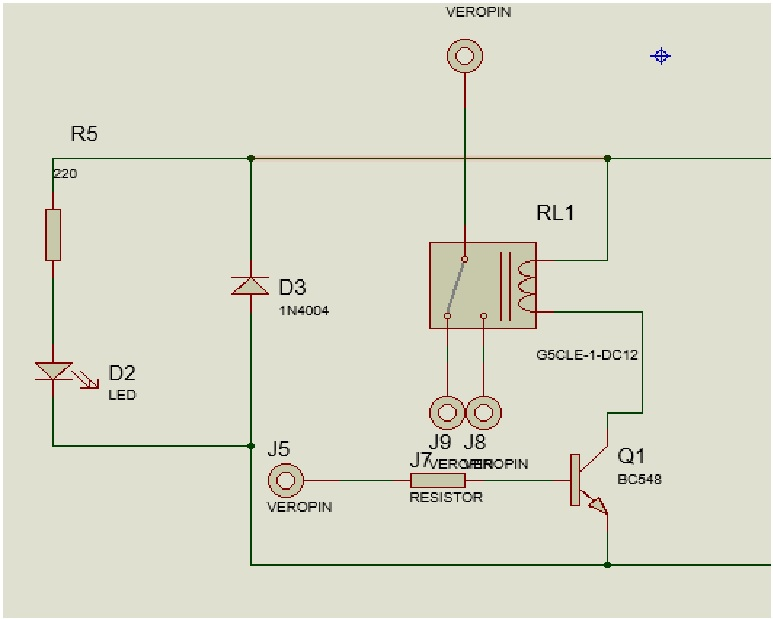
\includegraphics[width=16cm]{figuras/controletemperatura_eletronica.jpg}
\caption{Diagrama Eletrônico de Controle de Temperatura.}
\end{figure}

O transistor BC548 atua como uma chave, que por sua vez é ativada com uma corrente advinda do MSP430, o que faz com que o caminho da corrente seja liberado e a corrente percorra o indutor presente no relé, gerando um fluxo magnético capaz de acionar o mesmo. Será utilizado também um Light Emitting Diode (LED), afim de indicar quando o sistema está ligado e um diodo de silício para que uma corrente reversa seja evitada. 
Quando o sistema estiver a uma temperatura acima de 4ºC, o compressor é ligado e quando o sistema atingir uma temperatura de 2ºC ou menor, o compressor é desligado, mantendo essa temperatura entre 2ºC e 4ºC.

\subsection{Sistema de proteção de componentes elétricos e eletrônicos}

Devido ao grau de confiabilidade que o produto construído demanda, por ser um sistema de transporte de órgãos para transplante, têm-se que instalar diversos circuitos de proteção de componentes, garantindo assim o perfeito estado e funcionamento dos componentes internos. 

Para isso será utilizado um circuito de proteção contra sobretensão com base em um SRC ou diodo controlado de silício. Este componente é muito importante em aplicações que possuem o objetivo de controlar cargas de potência de altos valores a partir da rede de energia.

Sendo assim, desenvolveu-se uma topologia de circuito utilizando o regulador de tensão LM7805 para estabilizar em 5Vdc e utilizar um diodo zener de proteção para estabilizar a tensão abaixo de 5.1Vdc. Caso ocorra uma sobrecarga de tensão no circuito, o diodo zener passará a conduzir corrente acionando os 2 SRCs e consequentemente queimando o fusível de proteção.

Pode-se observar na imagem abaixo o esquemático do circuito a ser implementado:

\begin{figure}[H]
\centering
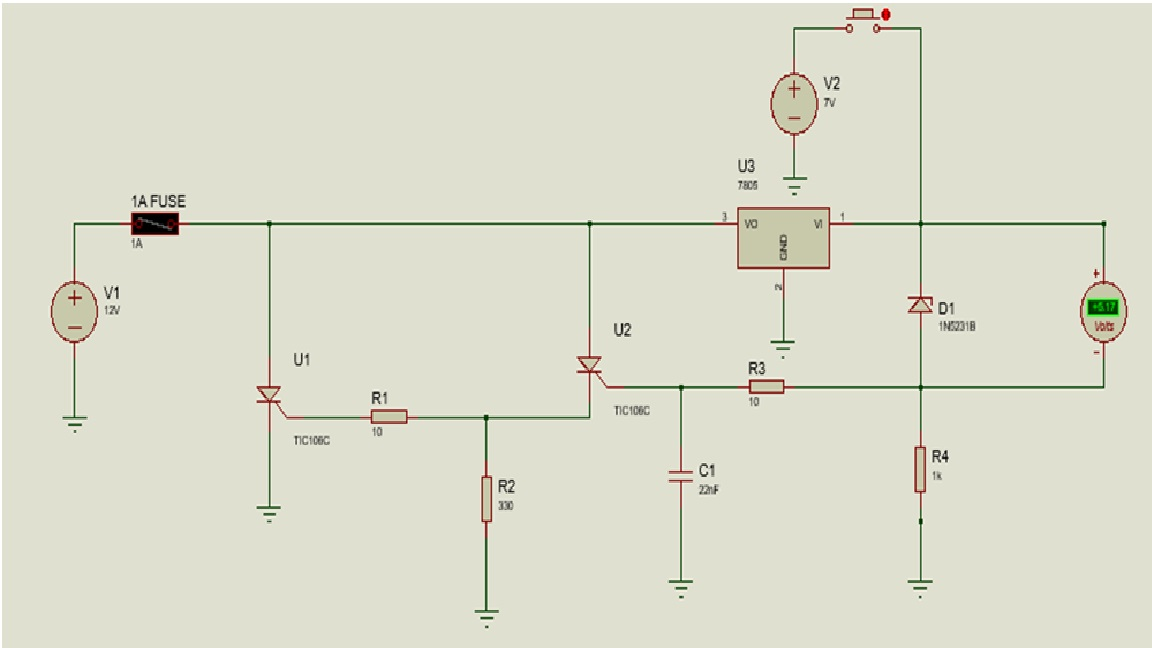
\includegraphics[width=16cm]{figuras/circuitoprotecao_eletronica.jpg}
\caption{Circuito de proteção.}
\end{figure}

Neste caso, pode-se observar uma fonte de 7V acoplada a um botão que simula uma sobretensão, 2 SRCs que são ativados quando o zener sobre uma sobretensão  causando a abertura do SRC U1 e consequentemente ativando o fusível. Desta forma,  garantisse  a proteção satisfatória dos componentes
	
Após a simulação, foram realizados testes de prototipagem em protoboard. Em seguida, depois da verificação da funcionalidade do sistema a nível de prototipagem, foi dimensionado o layout do circuito para realizar a confecção da PCB por meio de serigrafia e corrosão no percloreto de ferro.


\begin{figure}[H]
\centering
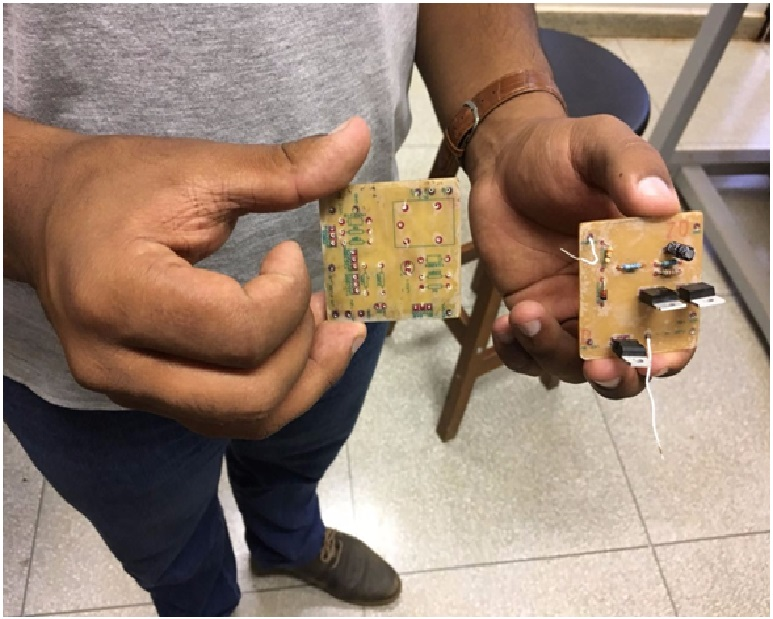
\includegraphics[width=16cm]{figuras/demonstracao_eletronica.jpg}
\caption{Placas eletrônicas.}
\end{figure}

Por fim foram realizados testes utilizando uma fonte de bancada e setando sua entrada em 12 V DC, neste caso foi observada  uma saída de 4.71V suficiente para alimentar tanto a raspberry PI quanto o MSP430.


\begin{figure}[H]
\centering
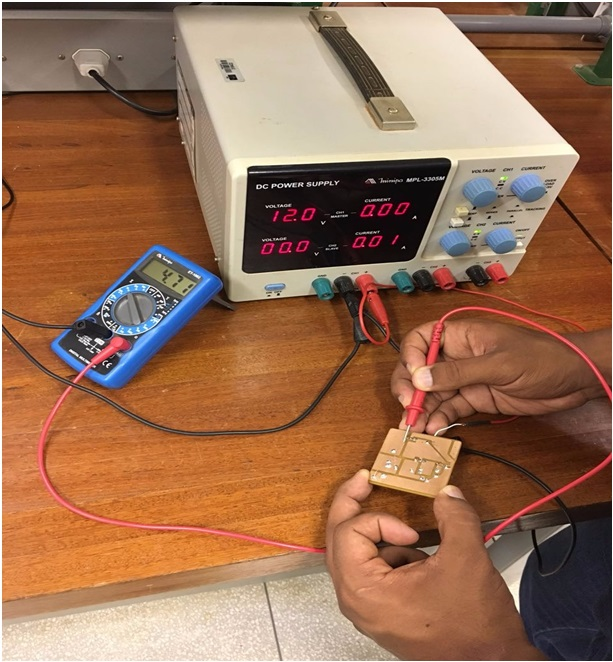
\includegraphics[width=16cm]{figuras/testedebancada_eletronica.jpg}
\caption{Testes de bancada com as placas fabricadas.}
\end{figure}

